\section{Eksperimentinis tyrimas}\label{sec:experiment}

\subsection{Tyrimo aprašymas}
Naudodami \refFramework{MalGAN} \glswhat{framework} paruošime
\glswhat{adversarial} ir apskaičiuosime jų efektyvumą prieš komercinius
detektorius.

\subsubsection{\acs{gan} implementacija} Naudosime \href{https://github.com/ZaydH/MalwareGAN}{viešai
    \textit{Github} platformoje
    paskelbtą\footnote{https://github.com/ZaydH/MalwareGAN}} \textit{MalGAN}
karkaso \acs{ml} modelio implementaciją.
% Generatoriaus nuostolių funkciją
% modifikuosime taip:

% \begin{equation}
%     L_G = \mathbb{E}_{m \in S_{Malware}, z\sim p_{\mathcal{N}^*(0,1)}}\log{D(G(m,z))}
% \end{equation}

% čia $z$ -- normalizuotas \enquote{triukšmo} pagal Gauso skirstinį ($\mathcal{N}^*(0,1)$) vektorius (Hu et~al. naudoja tolygų skirstinį).

\subsubsection{\acs{gan} mokymosi duomenys} Mokymuisi naudosime \textit{EMBER}
\cite{andersonEMBEROpenDataset2018a} duomenų rinkinį. Treniravimo aibė susideda
iš $2000$ programų požymių (\textit{API} vardų iš \textit{ImportTable} \acs{pe}
formato failo sekcijos). Aibė subalansuota -- joje yra po $1000$ kenkėjiškų ir
nekenkėjiškų programų požymių. Mokymosi etapui taip pat taikysime treniravimo /
validacijos skaidinį santykiu $4:1$.

\subsubsection{\Glswhom{framework} parametrai}
\begin{itemize}
    \item Dvejetainio požymių vektoriaus $M$ dimensija $d_M = 10000$
    \item \enquote{Triukšmo} vektoriaus $Z$ dimensija $d_Z=100$
    \item Neuronų skaičius generatoriaus \enquote{paslėptuose} sluoksniuose:
          $100,256,512,1024$
    \item Neuronų skaičius diskriminatoriaus \enquote{paslėptuose} sluoksniuose:
          $256,256$
    \item Diskriminatoriaus mokymosi greitis $\alpha_D = 4\cdot 10^{-4}$
    \item Generatoriaus mokymosi greitis $\alpha_G = 10^{-6}$
\end{itemize}

\subsubsection{Realių kenkėjiškų programų rinkinys}\label{sec:experiment:virusshare}
Atakoms naudosime realias kenkėjiškas \acs{pe} formato programas iš
\href{https://virusshare.com/}{\textit{VirusShare}\footnote{https://virusshare.com/}}.
Duomenų rinkinį sudaro $100$ kenkėjiškų programų.

\subsubsection{Komerciniai detektoriai}
Tiek originalias, tiek modifikuotas (\acs{ae}) kenkėjiškas programas
patikrinsime su
\href{https://www.virustotal.com}{\textit{VirusTotal}\footnote{https://www.virustotal.com}}
-- paslauga, kuri agreguoja daugiau nei $70$ komercinių kenkėjiškų programų
detektorių.

\clearpage
\subsection{Mokymosi etapas}

Specifinis \refFramework{MalGAN} mokymosi etapas yra tokia seka:
\begin{enumerate}
    \item Išmokomas \enquote{juodos dėžės} modelis (šiuo atveju pasirinktas
          \enquote{atsitiktinio miško} (\angl{random forest}) modelis).
    \item Mokoma pagal bendrą seką (aptartą \ref{sec:literature:gan}), kurioje:
          \begin{itemize}
              \item Praleidžiamas originalios programos perturbacijos žingsnis (diskriminatoriui
                    iškart perduodamas \acs{ae} požymių vektorius).
              \item Generatorius ir diskriminatorius mokomi kartu, kadangi diskriminatorius turi
                    naudoti generatoriaus sugeneruotus \acs{ae}, o generatoriaus nuostolių funkcija
                    priklauso nuo diskriminatoriaus išvesties. Šis žingsnis pavaizduotas
                    \ref{fig:experiment:learning}-ame pav.
          \end{itemize}
\end{enumerate}

\begin{figure}[h]
    \begin{small}
        \begin{center}
            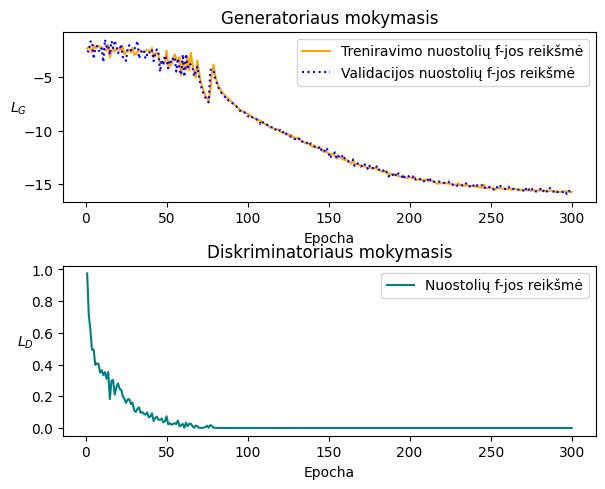
\includegraphics[width=0.95\textwidth]{img/learning.png}
        \end{center}
        \caption{\textit{MalGAN} generatoriaus ir diskriminatoriaus nuostolių funkcijų reikšmės mokymosi etape}\label{fig:experiment:learning}
    \end{small}
\end{figure}

\subsection{Varžymosi principais pagrįstos atakos prieš komercinius detektorius}

Naudodami mokymosi etape ištreniruotą \acs{ml} modelį ir
\ref{sec:experiment:virusshare} aptartą duomenų rinkinį, sugeneruosime \acs{ae}
ir palyginsime, kiek komercinių detektorių aptinka originalias programas
($N_{orig}$) ir kiek obfuskuotas pagal \textit{MalGAN} karkasą ($N_{adv}$).

Atakų efektyvumą $\mu$ skaičiuosime remiantis Zhong et~al. pasiūlyta formule
$\mu' = \frac{N_{orig} - N_{adv}}{N_{orig}}$
\cite{zhongMalFoxCamouflagedAdversarial2024}, laikydami, jog atakos efektyvumas
neneigiamas $\mu = \max{(\mu', 0)}$.

\begin{figure}[h]
    \begin{small}
        \begin{center}
            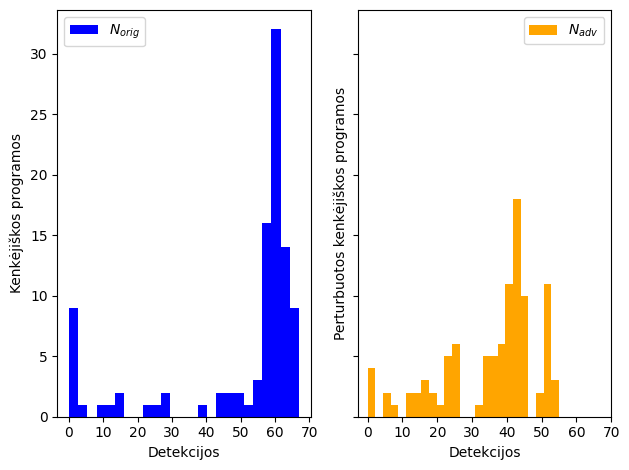
\includegraphics[width=0.6\textwidth]{img/det_distributions.png}
        \end{center}
        \caption{Originalių ($N_{orig}$) ir perturbuotų ($N_{adv}$) kenkėjiškų programų detekcijų pasiskirstymas}\label{fig:experiment:det_dist}
    \end{small}
\end{figure}

\begin{figure}[h]
    \begin{small}
        \begin{center}
            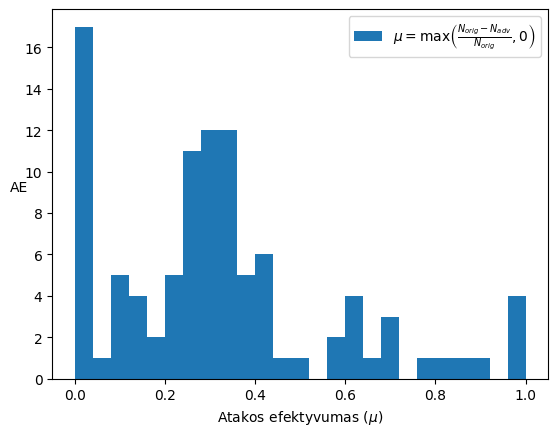
\includegraphics[width=0.6\textwidth]{img/mu_distribution.png}
        \end{center}
        \caption{\Glswhose{adversarial} efektyvumo pasiskirstymas}\label{fig:experiment:mu_dist}
    \end{small}
\end{figure}

\begin{tabular}{ll}
    \textbf{Efektyvumo vidurkis}:    & $26,85\%$ \\
    \textbf{Standartinis nuokrypis}: & $18,97\%$
\end{tabular}